%[In the next chapters I describe the overall characteristics and limitations that a VLC system should present according to my findings, identify the variables involved and the set of parameters necessary for it to work. This chapter should provide a useful starting point for whoever plans to implement one in practice What does one need to make his own VLC system?]
%Structure of a VLC system: logical layer, control layer, physical layer. Analysis and characteristics of the three.
%logical abstraction
Every visible light communication system shares the same underlying structure, as also general other communication systems.
Communication needs to be established between two ends, one end that acts as a transmitter and the other that acts as a receiver.
There are at least three levels of abstraction needed to transform a digital information into a signal that can be sent and received, and these can be defined as: 
\begin{itemize}
\item \textbf{logical layer}, where the information is handled at a software level
\item \textbf{control layer}, responsible of managing the variations of the physical property used for communication in a organised and structured manner
\item \textbf{physical layer}, where the properties of the communication are limited by the physical properties of the signal and the characteristics of the hardware
\end{itemize}
Each of these levels present different characteristics that combined form the overall performance of the system.\\

%physical
In VLC, the transmitter end of the communication operates on a light emitter to vary a property of the light depending on the modulation scheme used (see \ref{modulschemes}), like brightness or colour.
The receiver on the other end needs to be able to detect such variations in a measurable manner.
This level can be described as the \textbf{physical layer} of the communication.
At this level, the system's performance can be influenced by physical properties of the hardware, like maximum brightness of the light emitter, warmup time intended as the time that the emitter takes to turn on, but also by other factors, like distance between the two ends, the medium of transmission, the angle of incidence of the light between transmitter and receiver and so on.\\

%control
These variations in the properties of light need to be controlled and organised to carry specific information.
A \textbf{control layer} is necessary in order to make the link between logical information and variation of physical property.
This layer is of critical importance for the performance of any system, since it influences the frequency of the physical variations which results in the rates for transmission and reception.
Factors that are to be considered in this layer are directly linked to the hardware components, namely any characteristic that influences the overall speed of transmission/reception, like clock rates of the micro controllers, speed of the transistors used and so on.\\

%logical
The outer most level of abstraction is the \textbf{logical layer}, where information is handled and manipulated at a software level.
For a transmitter, this layer produces the instructions to deliver to the control layer in order to generate a signal given a specific information. 
This process can be seen as the logical encoding of the information, ready to be transferred and become physical encoding.
At the opposite end of the transmission, the logical layer of a receiver is given data about physical variations measured by the sensor(s) used in the system, and needs to reconstruct and interpret such data back to the original information.
Contrary to the previous layers, the performance of the logical layer doesn't rely much on the hardware and the physical characteristics of the components, but rather on the software techniques and algorithms that implement it.
A well structured logical layer could potentially add more reliability to an otherwise uncertain medium of communication, allowing a stricter control on the traffic and implementing recovery options in case of mistakes.

\begin{figure}[hbt]
  \centering
  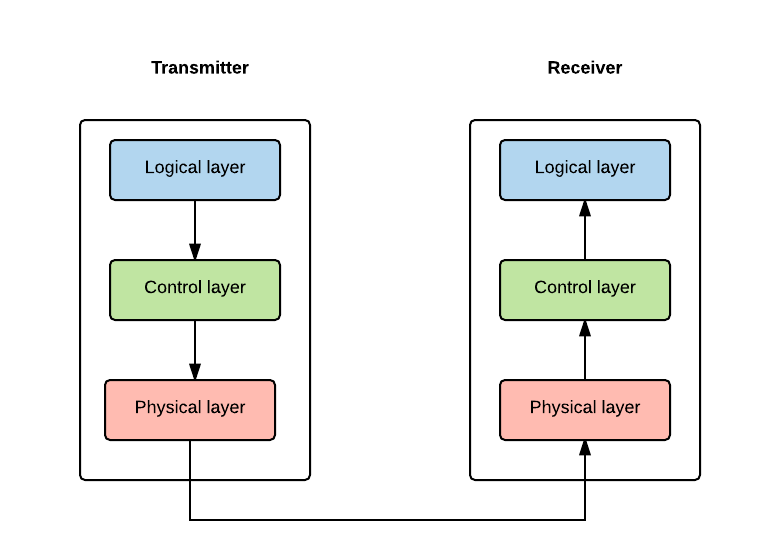
\includegraphics[height=180px]{img/LCP}
  \caption{Conceptual layers of the system.}
  \label{fig:lcp}
\end{figure}


%prototype architecture
\subsection{Experimental setup}
\label{expsetup}
In order to verify feasibility, investigate characteristics and test performance of general VLC systems, a prototype system has been developed.
The system is composed of two main modules: a transmitter module, and a receiver.
The transmitter module uses On Off Keying with Manchester Coding (see \ref{modulschemes})  to convey signals through light.
In order to allow testing, this module takes some arbitrary input from a user, encapsulates the information and encodes it to produce variations in light intensity, through the control of a light emitter.
The receiver side measures the light variations through the use of a photoresistor, a sensor that measures light intensity, reconstructing and interpreting the sensor data back into the original messages. 
If the message that is received matches the one that is sent, the communication is considered successful.
Each module includes different components, listed in section \ref{components}.
Fig. \ref{fig:sys over} shows an overview of the prototype's architecture.

\begin{figure}
\centering
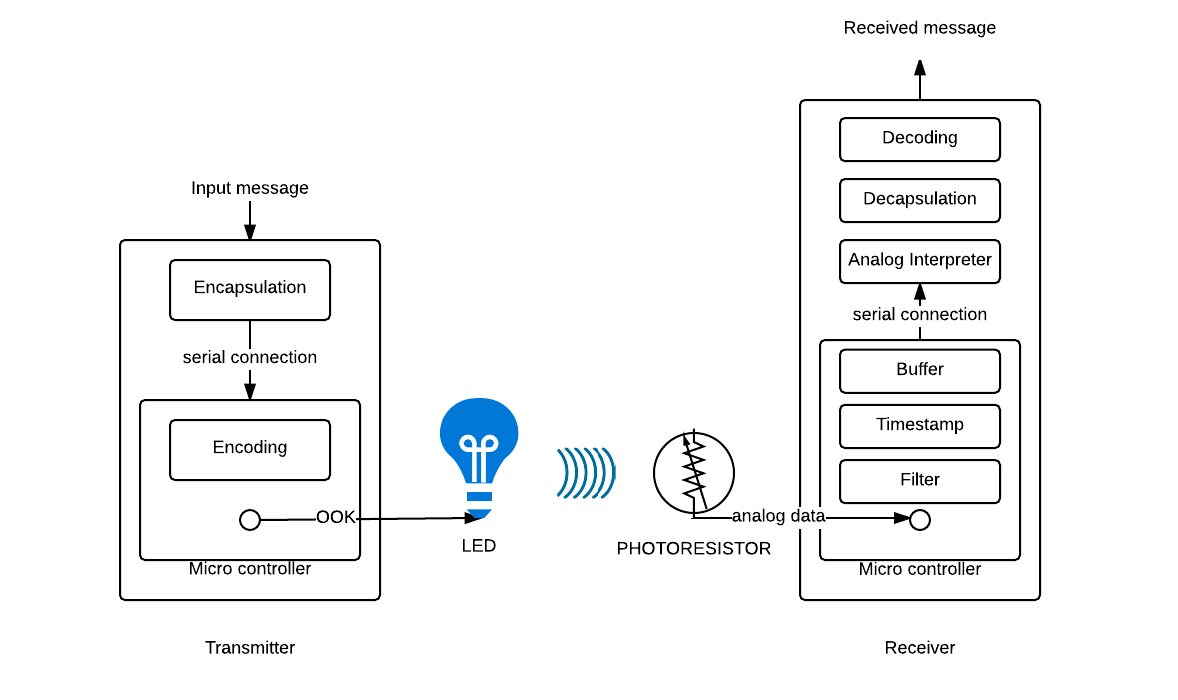
\includegraphics[height=200px]{img/sysover}
\caption{Prototype system.}
\label{fig:sys over}
\end{figure}

%transmitter
\subsubsection{Transmitter}
Transmission starts from a terminal, where a user can input messages as strings. These are then encapsulated into Protocol Data Units (PDUs) and sent to a micro controller through a serial connection.
In this case, the micro controller that was used for transmission is an Arduino board.
The board encodes the received bytes into Manchester Code, and then controls the light signal by switching on and off the emitter accordingly.
The Manchester encoding allows the light emitter to always produce some base illumination regardless of the data sent. 
If the message to be sent in binary consisted of a long sequence of binary 0s, a pure binary encoding would result in the light being turned off for the entire time.
Instead, Manchester encoding constantly alternates the symbols, employing in average the same amount of states with light on and states with light off.
A light emitting diode is the furthest end of the transmitter module.
For this part, multiple setups have been tried.
The fastest emitter that has been tested is a single low power bright LED connected to the board and powered directly by it, which allows very fast switching.
The LED is 10 mm wide and has an optimal viewing angle of about $30^{\circ}$.
The brightness achieved by this LED is enhanced through the use of a lens.
%LEDs are preferable compared to incandescent or fluorescent light bulbs, since they are generally faster and are not damaged by the switching like the other options.
%All other kinds of bulbs, halogen, incandescent and fluorescent, have tungsten filaments that get damaged by the thermal shock of the switching, so they require more time, more power and do not last as long if compared to LEDs.
A second setup has also been tested with a commercial LED bulb powered by an external power source (mains electricity), and controlled by the board through a switcher. 
A bigger bulb, energised with a high power source, can achieve greater luminous intensity and reach longer distances.
The bulb can reach up to 240 lumen at a $120^{\circ}$ viewing angle.
However controlling external power sources is lightly more complex, and especially so with alternating current as in the case of mains electricity.
This second setup with the LED light bulb was not used in the final stages to achieve communication, for various limitations encountered in the process.
Most of the results achieved later on will be referring to the first setup with the fast switching low power LED, unless otherwise specified.

%receiver
\subsubsection{Receiver}
The signal is received by a photodiode and read as analog input by a micro controller.
On the board, values are software-filtered to reduce noise, and sent to the receiving terminal with a timestamp.
The board and the terminal are connected through a serial connection.
Some controllers could read directly analog input and perform the remaining processes to interpret the signal, with enough computational power.\\ 
For this application, the final terminal is a Raspberry Pi, since it has a good power/size ratio for the designed purpose and allows a simple prototyping process. The micro controller in between the sensor and the terminal is necessary to read and forward analog data, which is not possible directly from the Raspberry Pi.\\
On the final terminal, the variations of sensory data are interpreted as sequences of digital 0s and 1s, finally decapsulated and decoded back into a message.

%components
\subsection{List of components}
\label{components}
Each module of the prototype system is composed of different components, listed in the following.\\
Transmitter:
\begin{enumerate}
\item personal computer as main terminal for user input and information processing
\item Genuino Uno micro controller board, based on ATmega328P \cite{genuinouno}
\item Light emitting diodes:
\begin{enumerate}
\item low power super bright LED, Blue 10 mm, forward voltage 3.0-3.4VDC, luminosity of 8 000-10 000 MCD, directional, 30$^{\circ}$ viewing angle \cite{ledDS}
\item commercial LED bulb, 230 V AC, 3 W, 240 lumen, directional, 120$^{\circ}$ viewing angle 
\end{enumerate}
\item Solid State Relay for Arduino, 5V activation, 240V load
\end{enumerate}
Receiver:
\begin{enumerate}
\item Photoconductive Cell VT900
\item Genuino Yun micro controller board, based on ATmega32u4 \cite{arduinoyun}
\item Terminals:
\begin{enumerate}
\item personal computer for test of communication
\item Raspberry Pi 3 Model B to be applied on a mobile robot \cite{raspberrypi}
\end{enumerate}
\end{enumerate}

\subsection{Wiring}
In figure \ref{fig:wiringDC} is shown the wiring of all the components of the prototype system.

\begin{figure}[hbt]
\centering
  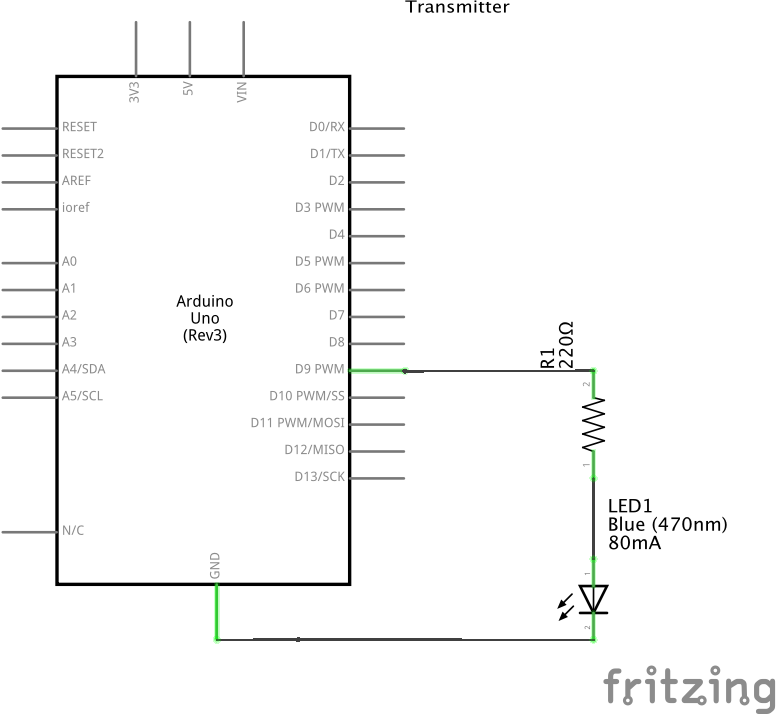
\includegraphics[height=150px]{img/transmitter_schem1}
  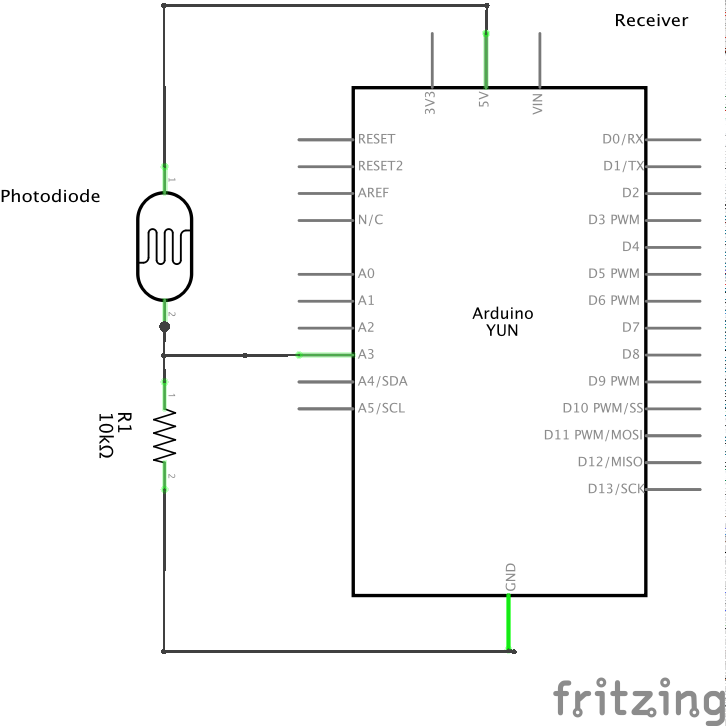
\includegraphics[height=150px]{img/receiver_schem1}
  \caption{Wiring of the boards and sensors.}
  \label{fig:wiringDC}
\end{figure}


